\chapter{Derivation of the current dipole approximation}
\label{app:dipoleappendix}
A volume containing a set of current sinks and sources will set up an electric potential given by the following equation:
\begin{equation}\label{eq:point_source}
\Phi(\mathbf{r}) = \frac{1}{4 \pi \sigma} \sum_{k=1}^N \frac{I_k}{|\mathbf{r} - \mathbf{r}_k|},
\end{equation}
where $I_k$ is the current in location ${\bf r}_k$ giving the electric potential $\Phi$ at electrode location ${\bf r}$.

From this, we outline the current dipole approximation, as an approximate alternative to the precise equation above.

\section{Current multipole expansion}
Analogous to how we can formulate the electric potential from a set of electric charges with the charge multipole expansion, we can similarly derive the current multipole expansion for a set of currents.

We picture $N$ currents $I_k$ located at $\mathbf{r}_k$ in a volume centered around position $\mathbf{r}_c = \sum_{k = 1}^N \frac{\mathbf{r}_k}{N}$. Our measurement electrode is positioned a distance $R = |\mathbf{R}| = |\mathbf{r}_c - \mathbf{r}|$ away from the current distribution, see Fig.~\ref{fig:current_volume}.

\begin{figure}[!ht]
	\begin{center}
		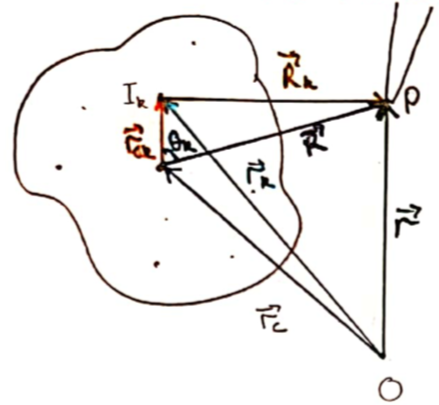
\includegraphics[width=0.3\textwidth]{Figures/placeholder_appB1.png}
	\end{center}
	\caption{\textbf{Placeholder: Electric potential from volume containing current sinks and sources}}
	\label{fig:current_volume}
\end{figure}

Our first step is to write $\frac{1}{|{\bf r} - {\bf r}_k|} = \frac{1}{R_k}$ from Eq.~\ref{eq:point_source} as an infinite series. Here, $R_k$ is the distance between current $I_k$ at ${\bf r}_k$ and the electrode position ${\bf r}$.

We start by applying the cosine rule,
\begin{equation}\label{eq:cos}
R_k^2 = R^2 + r_{ck}^2 - 2 R r_{ck} \cos \theta_k.
\end{equation}
where $r_{ck} = |{\bf r}_{ck}|$ is the length of the distance vector between the volume mid point ${\bf r}_c$ and current location ${\bf r}_k$, and $\theta_k$ is the angle between ${\bf r}_{ck}$ and ${\bf R}$, see Fig.~\ref{fig:theta_k}.

\begin{figure}[!ht]
	\begin{center}
		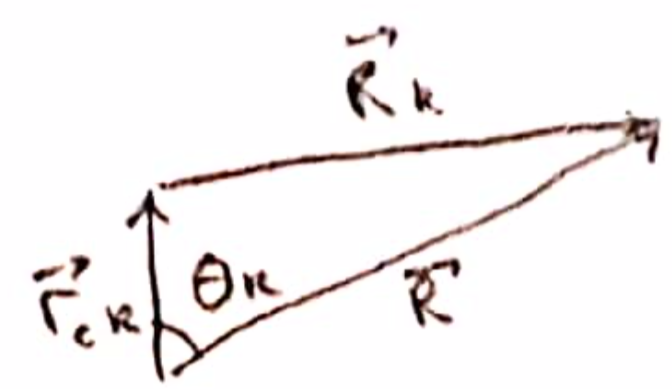
\includegraphics[width=0.3\textwidth]{Figures/placeholder_appB2.png}
	\end{center}
	\caption{\textbf{Placeholder: Angle between ${\bf r}_{ck}$ and ${\bf R}$}}
	\label{fig:theta_k}
\end{figure}

Further, we rewrite Eq.~\ref{eq:cos} above to get the following expression for $R_k$:

\begin{align*}
R_k^2 &= R^2\big[1 -  \frac{r_{ck}}{R} 2 \cos \theta_k + \big(\frac{r_{ck}}{R}\big)^2  \big] \\
\implies R_k &= R\sqrt{1 - 2 h \cos \theta_k + h^2} \quad \forall h = \frac{r_{ck}}{R}
\end{align*}

%
This means that we can write:

\begin{equation*}
\frac{1}{|{\bf r} - {\bf r}_k|} = \frac{1}{R\sqrt{1 - 2 h \cos \theta_k + h^2}}
\end{equation*}

Noticing that $\frac{1}{\sqrt{1 - 2 h \cos \theta_k + h^2}}$ is the generating function for the Legendre polynomials, we find that

\begin{align*}\label{eq:legendre}
\frac{1}{\sqrt{1 - 2h\cos \theta_k + h^2}} &= \sum_{l = 0}^\infty h^l P_l(\cos \theta_k) \quad \quad \quad \forall \quad |h| = |\frac{r_{ck}}{R}| < 1 \\
\implies \frac{1}{|{\bf r} - {\bf r}_k|} &= \frac{1}{R} \sum_{l = 0}^\infty \big(\frac{r_{ck}}{R}\big)^l P_l(\cos \theta_k) \quad \quad \forall \quad R > r_{ck}.
\end{align*}
Here, $P_l$  are the Legendre polynomials, such that:
\begin{align*}
P_0 (\cos \theta_k) &= 1 \\
P_1 (\cos \theta_k) &= \cos \theta_k \\
P_2 (\cos \theta_k) &= \frac{3}{2} \cos^2 \theta_k - \frac{1}{2} \\
P_3 (\cos \theta_k) &= \frac{5}{2} \cos^3 \theta_k - \frac{3}{2}\cos \theta_k \\
&\;\;\vdots \notag
\end{align*}

Inserting our infinite series expression for $\frac{1}{|{\bf r} - {\bf r}_k|}$ into Eq.~\ref{eq:point_source}, we arrive at the current multipole expansion:

\begin{equation}\label{eq:multipole_compact}
\Phi (R) = \frac{1}{4 \pi \sigma}\frac{1}{R} \sum_{k=1}^N I_k \sum_{l = 0}^\infty \big(\frac{r_{ck}}{R}\big)^l P_l(\cos \theta_k) \quad \forall~ R > r_{ck}.
\end{equation}

Writing out the first terms, we find that

\begin{align}\label{eq:multipole}
\Phi(R) =~& 
\frac{1}{4 \pi \sigma} \Bigg[\frac{1}{R} \sum_{k=1}^N I_k \nonumber\\
&~~~~+ \frac{1}{R^2} \sum_{k=1}^N I_k r_{ck} \cos \theta_k \\
&~~~~+  \frac{1}{R^3} \sum_{k=1}^N I_k r_{ck}^2 \left( \frac{3}{2} \cos^2 \theta_k - \frac{1}{2} \right) \nonumber \\
&~~~ +  \frac{1}{R^3} \sum_{k=1}^N I_k r_{ck}^3 \left( \frac{5}{2} \cos^3 \theta_k - \frac{3}{2} \cos \theta_k \right) ... \nonumber \Bigg] \quad \forall R > r_{ck}.
\end{align}

Here, the first four terms are known as the monopole $\Phi^{\mathrm{mono}}$, dipole $\Phi^{\mathrm{dipole}}$, quadrupole $\Phi^{\mathrm{quadrupole}}$ and octopole $\Phi^{\mathrm{octopole}}$ contributions, respectively, such that

\begin{equation}
\Phi = \Phi^{\mathrm{monopole}} + \Phi^{\mathrm{dipole}} + \Phi^{\mathrm{quadrupole}} + \Phi^{\mathrm{octopole}} + ...
\end{equation}

Now, we are going to take a look at how the first four terms of the current multipole expansion contribute to the extracellular potential in neural tissue.

\section{Monopole contribution in neural tissue}\label{subsec:mono}
Due to current conservation in neural tissue, the transmembrane current sinks and sources for a whole number of neurons will always sum to zero: $\sum_k I_k = 0$. This means that the monopole contribution term will always be zero in neural tissue:

\begin{equation*}
\Phi^{\mathrm{monopole}} = \frac{1}{4 \pi \sigma} \frac{1}{R} \sum_k I_k = 0
\end{equation*}

\section{Dipole contribution in neural tissue/ the current dipole approximation}
The dipole contribution is given as 
\begin{equation*}
\Phi^{\mathrm{dipole}} = \frac{1}{4 \pi \sigma} \frac{1}{R^2} \sum_k I_k r_{ck} \cos \theta_k
\end{equation*}
Applying the definition of the scalar product ${\bf r}_{ck} \cdot {\bf R} = r_{ck} \text{R} \cos \theta_k$, we see that $r_{ck} \cos \theta_k = {\bf r}_{ck} \cdot {\bf \hat{R}}$, where $\hat{{\bf R}} = {\bf R}/\text{R}$ , we can write the expression above as follows:

\begin{align*}
\Phi^{\mathrm{dipole}} &= \frac{1}{4 \pi \sigma} \frac{1}{R^2} \sum_k I_k {\bf r}_{ck} \cdot {\bf \hat{R}} \\
		   &= \frac{1}{4 \pi \sigma} \frac{1}{R^2} \sum_k I_k ({\bf r}_{k} - {\bf r}_{c}) \cdot {\bf \hat{R}} \\
 		   &= \frac{1}{4 \pi \sigma} \frac{1}{R^2} \left(\sum_k I_k {\bf r}_{k} \cdot {\bf \hat{R}} - \sum_k I_k {\bf r}_{c} \cdot {\bf \hat{R}} \right)
\end{align*}
Since $\sum_k I_k {\bf r}_k = {\bf p}$ and $\sum_k I_k = 0$, we here end up with the current dipole approximation:

\begin{equation}
\Phi \approx \Phi^{\mathrm{dipole}} = \frac{1}{4 \pi \sigma} \frac{{\bf p} \cdot {\bf \hat{R}}}{\text{R}^2} = \frac{1}{4 \pi \sigma} \frac{\text{p} \cos \theta}{R^2},
\end{equation}

Here, $\theta$ is the angle between ${\bf p}$ and ${\bf R}$. Since the current dipole approximation is based on the multipole expansion, the constraint $\text{R} > r_{ck}$ still holds.

In \ref{subsec:mono}, we saw that there are no monopole contributions to electric potentials from a whole number of neurons. However, applying the current-dipole approximation, we neglect the higher-order terms in the current multipole expansion, which calls for stricter constraints: $R >> r_ck$. In order to get an intuition about when $R$ is "large enough", we will look into the quadrupole and octopole contributions ($\Phi^{\mathrm{quadrupole}}$, $\Phi^{\mathrm{octopole}}$) from a single current sink and a current source.

\section{Quadrupole contribution from a single current sink source pair}\label{subsec:quad}

From Eq.~\ref{eq:multipole}, we see that the quadrupole contribution for a current sink $I_1$ at $r_1$ and a current source $I_2$ at $r_2$ is

\begin{equation}\label{eq:phi_quad}
\Phi^{\mathrm{quadrupole}} = \frac{1}{R^3} \left[ I_1 r_{c1}^2 \left( \frac{3}{2} \cos^2 \theta_1 - \frac{1}{2} \right) + I_2 r_{c2}^2 \left( \frac{3}{2} \cos^2 \theta_2 - \frac{1}{2} \right) \right].
\end{equation}

When the center of the volume is defined halfway between the sink and the source $I_2 = -I_1$, we know that $r_{c1} = r_{c2}$, and that

\begin{align*}
\theta_2 &= \pi - \theta_1 \\
\implies \cos \theta_2 &= -\cos \theta_1 \\
\implies \cos^2 \theta_2 &= \cos^2 \theta_1.
\end{align*}

Inserting this into \eqref{eq:phi_quad}, we see that $\Phi^{\mathrm{quadrupole}} = 0$, meaning that there is no quadrupole contribution to the extracellular potential from a sink-source pair.

Since all terms of Legendre polynomials for $l = 4, 6, 8, ...$ contain $\cos \theta_k$ raised to the power of an even number, multipole expansion term number 3, 5, 7, 9, etc are all equal zero for a sink-source pair.

\section{Octopole contribution from a single current sink source pair}\label{subsec:octo}

For a sink-source current pair, $I_1$ at ${\bf r}_1$ and $I_2$ at ${\bf r}_2$, we have the following octopole contribution:

\begin{equation*}
\Phi^{\mathrm{octopole}} = \frac{1}{4 \pi \sigma} \frac{1}{R^4}\left[ 
I r_{c1}^3 \left( \frac{5}{2} \cos^3 \theta_1 - 
\frac{3}{2}\cos \theta_1 \right) - 
I r_{c2}^3 \left( \frac{5}{2} \cos^3 \theta_2
 - \frac{3}{2} \cos \theta_2 \right)
\right].
\end{equation*}

If ${\bf r}_{c}$ is the midpoint between ${\bf r}_1$ and ${\bf r}_2$, we can say that $r_{c2} = r_{c1} = \frac{d}{2}$ and $\cos \theta_2 = - \cos \theta_1$. This implies that

\begin{align*}
\Phi^{\mathrm{octopole}} &= \frac{1}{4 \pi \sigma} \left[
I \frac{d}{2}^3 \left( \frac{5}{2} \cos^3 \theta_1 - 
\frac{3}{2}\cos \theta_1 \right) - 
I \frac{d}{2}^3 \left( \frac{5}{2} \cos^3 \theta_1
 - \frac{3}{2} \cos \theta_1 \right)
\right] \\
&= \frac{1}{4 \pi \sigma} \frac{I d^3}{R^4} \frac{1}{16} \left(
5 \cos^3 \theta_1 - 3 \cos \theta_1 + 5 \cos^3 \theta_1 - 3 \cos \theta_1
\right) \\
&= \frac{1}{4 \pi \sigma} \frac{I d^3}{R^4} \frac{5 \cos^3 \theta_1 - 3 \cos \theta_1}{8}
\end{align*}

For a single current sink source pair $\theta_1 = \theta$, where $\theta$ is the angle between ${\bf p}$ and ${\bf R}$, such that

\begin{align*}
\Phi^{\mathrm{octopole}} = \frac{1}{4 \pi \sigma} \frac{p}{R^2} \frac{d^2}{R^2} \frac{5 \cos^3 \theta - 3 \cos \theta}{8}.
\end{align*}

Including the octopole contribution when estimating the extracellular potential from a sink-source pair, as opposed to applying the current dipole approximation, can be quantified as follows:

\begin{equation*}
\big| \frac{\Phi^{\mathrm{octopole}}}{\Phi^{\mathrm{quad}}} \big|_{\mathrm{max}} = \big|\frac{d^2}{R^2} \frac{5 \cos^2 \theta - 3}{8}\big|_{\mathrm{max}} = \frac{3}{8} \frac{d^2}{R^2}
\end{equation*}

In \cite**{Nunez2006}, it is suggested that the current dipole approximation is applicable when $R > 3d$ or $R > 4d$.

For a sink-source pair, the octopole contribution is maximum $\Phi^{\mathrm{octo}}(R = 3d) = \frac{1}{24} \Phi^{\mathrm{dipole}}$ and $\Phi^{\mathrm{octo}}(R = 4d) = \frac{3}{128} \Phi^{\mathrm{dipole}}$.

%\snnote{current dipole approximation, suggestion 2}
%\slntxt{  
%	
%	In the next paragraph, we outline the current dipole approximation, as an alternative to eq.~\eqref{eq:VCtheory}. We picture $N$ currents $I_k$ located at $\mathbf{r}_k$ in a volume centered around position $\mathbf{r}_c = \sum_{k = 1}^N \frac{\mathbf{r}_k}{N}$. Our measurement electrode is positioned a distance $R = |\mathbf{R}| = |\mathbf{r}_c - \mathbf{r}|$ away from the current distribution.
%	
%	Starting out with eq.~\eqref{eq:VCtheory}, we can rewrite $\frac{1}{|\mathbf{r} - \mathbf{r}_k|}$ as a binomial expansion, by first applying the cosine rule. From this, we end up with an infinite series, better known as the multipole expansion for current sources:
%	
%	\begin{align}\label{eq:multipole}
%	\Phi(R) =~& 
%	\frac{1}{4 \pi \sigma} \Bigg[\frac{1}{R} \sum_{k=1}^N I_k \nonumber\\
%	&~~~~+ \frac{1}{R^2} \sum_{k=1}^N I_k r_k^c \cos \theta_k \\
%	&~~~~+  \frac{1}{R^3} \sum_{k=1}^N I_k r_k^{c~2} \left( \frac{3}{2} \cos^2 \theta_k - \frac{1}{2} \right) + ... \nonumber \Bigg]
%	\end{align}
%	
%	Where $r_k^c = |\mathbf{r}_k^c|$ is the distance between current source $k$ at position $\mathbf{r}_k$ and the distribution midpoint $\mathbf{r}_c$,
%	and $\theta_k$ is the angle between $\mathbf{r}_k^c$ and $\mathbf{R}$.
%	The multipole expansion gives us the exact potential at location $\mathbf{r}$, when $R > r_{k~max}$. Computing electric potentials applying the multipole expansion directly, is however not very useful, since we would need infinitely many terms.
%	Looking at the various terms in the multipole expansion, we notice that the terms decay with distance from the current distribution as $1/R$, $1/R^2$, $1/R^3$. The terms are often referred to as the \emph{monopole contribution}, the \emph{dipole contribution}, the \emph{quadrupole contribution}, etc, respectively.  For the case of a single current source, all terms but the monopole contribution, would give non-zero contributions to the electric potential. Due to current conservation, single current monopoles are unphysical in neural tissue.
%	The simplest current distribution that can result from neural activity is the current dipole, i.e. a current sink $I_1 = -I$ and a current source $I_2 = I$. Inserting this into the multipole expansion, we see that there is no monopole contribution, but the dipole contribution and higher-order terms will  contribute to the electric potential.
%	The dipole contribution from a single current dipole is known as the current dipole approximation and can be written on the form:
%	\begin{equation}\label{eq:CDA}
%	\Phi^{dipole}(\mathbf{R}) = \frac{1}{4 \pi \sigma} \frac{|\mathbf{p}| \cos \theta}{R^2},
%	\end{equation}
%	where $R = |\mathbf{r}_c - \mathbf{r}|$ is the distance from the midpoint of the so-called current dipole moment $\mathbf{p}$ to the electrode, and $\theta$ is the angle between $\mathbf{p}$ and $\mathbf{R}$.
%	
%	The current dipole moment from a current sink $I_1 = I$ and a current source $I_2 = -I$, located at position $\mathbf{r}_1$ and $\mathbf{r}_2$, respectively, can be calculated as
%\begin{align}\label{eq:p}
%\mathbf{p} &= I_1 \mathbf{r}_1 + I_2 \mathbf{r}_2 \nonumber\\
%&= I \mathbf{r}_1 - I \mathbf{r}_2 \\
%&= I \mathbf{d}, \nonumber
%\end{align}
%	
%	where $\mathbf{d}$ is the distance vector between the current sink and the current source, giving the length and direction of the dipole.
%	
%	Applying the current dipole approximation, we neglect the quadrupole and higher-order contributions to the electric potential. This is a good approximation in the far-field limit, that is when $R$ is much larger than the dipole length $d$, $R > 3d$ or $R > 4d$, since the higher-order terms decay rapidly with increasing distance \cite**{Nunez2006}.
%}
%
%\snnote{To be included for both suggestions:}
%
%\sntxt{
%	
%	It is important to note that when computing the electric potential in the far-field limit from a distribution of transmembrane currents in neural tissue, the dipole contribution will be the dominating term \cite**{Nunez2006}. By computing the total current dipole moment from a distribution of current sources
%	\begin{equation}
%	\mathbf{p} = \sum_{k=1}^N I_k \mathbf{r}_k,
%	\end{equation}
%	
%	we can approximate the electric potential from neural activity by applying the current dipole approximation.
%	
%	The point-source approximation, eq. \ref{eq:VCtheory} (or the line-source version of it), and the current dipole approximation, eq.~\eqref{eq:CDA} represent} volume conductor theory in its simplest form, and \sntxt{are} based on a set of assumptions, some of which may be relaxed for problems where it is relevant: 